\section{Resolução Questão 2}

% Slide 1: Enunciado da Questão
\begin{frame}[fragile]{Enunciado da Questão}
    Considere uma variável aleatória $X_i$ que segue uma distribuição Exponencial com parâmetro $\lambda = 3$.
    \vspace{1em}
    
    \begin{itemize}
        \item[\textbf{a)}] Gere $N = 10.000$ observações de $X_i$ e construa o histograma.
        \item[\textbf{b)}] Crie uma função ou linha de código que gere uma amostra de tamanho $n$ (ex: $n=2, 5, 50$) de $X_i$.
        \item[\textbf{c)}] Crie uma função ou linha de código que calcule a média de uma amostra de tamanho $n$.
        \item[\textbf{d)}] Para cada tamanho de amostra $n \in \{2, 5, 50\}$, gere 10.000 amostras e calcule a média de cada uma. Construa o histograma da distribuição dessas 10.000 médias amostrais ($\bar{X}$) para cada valor de $n$.
        \item[\textbf{e)}] Calcule a média e o desvio padrão das 10.000 médias amostrais ($\bar{X}$) para cada $n$.
        \item[\textbf{f)}] Com base nos resultados, enuncie o Teorema do Limite Central e explique como ele se aplica a este experimento.
    \end{itemize}
\end{frame}

% Slide 2: Histograma da alternativa 'a'
\begin{frame}{a) Histograma da Distribuição Original}
    \begin{figure}
        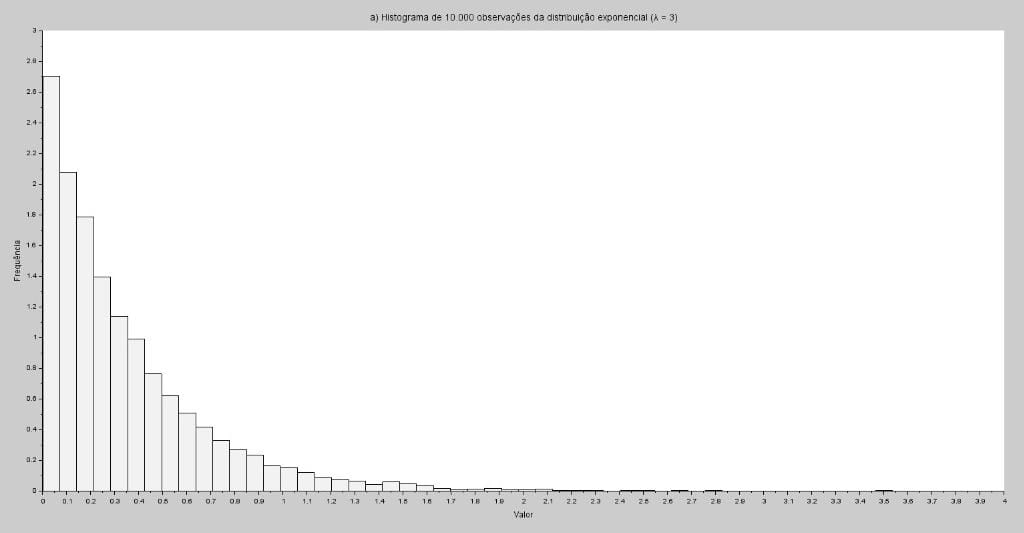
\includegraphics[width=0.85\textwidth]{figures/grafico1_dist_xi.jpg}
        \caption*{Gráfico 1: distribuição de Xi com n = 10000}
    \end{figure}
\end{frame}

% Slide 3: Código para 'b' e 'c'
\begin{frame}[fragile]{b) e c) Geração e Média de Amostras}
    \textbf{b) Crie uma função ou linha de código que gere uma amostra de tamanho $n$ de $X_i$.}
    \begin{lstlisting}
// O parametro da exponencial no Scilab e a media (1/lambda)
grand(1, n, "exp", 1/3)
    \end{lstlisting}
    Essa função cria a amostra com $n$ observações.
    
    \vspace{2em}
    
    \textbf{c) Crie uma função ou linha de código que calcule a média de uma amostra de tamanho $n$.}
    \begin{lstlisting}
mean(grand(1, n, "exp", 1/3))
    \end{lstlisting}
    Essa função calcula a média da amostra.
\end{frame}

% Slide 4: Código da alternativa 'd'
\begin{frame}[fragile]{d) Código para Gerar Médias Amostrais}
    \textbf{d) Para cada $n \in \{2, 5, 50\}$, gere 10.000 amostras e calcule a média de cada uma. Construa o histograma da distribuição dessas médias.}
    
\begin{lstlisting}
lambda = 3;
media_teorica = 1 / lambda;
N = 10000; // Número de amostras

// Gera 10.000 amostras (linhas) com n elementos (colunas)
Xn2 = grand(N, 2, "exp", media_teorica);
Xn5 = grand(N, 5, "exp", media_teorica);
Xn50 = grand(N, 50, "exp", media_teorica);

// Calcula a média de cada linha (amostra)
Xbar2 = mean(Xn2, 2);
Xbar5 = mean(Xn5, 2);

Xbar50 = mean(Xn50, 2);
\end{lstlisting}
\end{frame}

\begin{frame}[fragile]{d) Código para Gerar Médias Amostrais}
\begin{lstlisting}

// Código para plotar os histogramas (exemplo para n=50)
histplot(50, Xbar50);
xtitle("Histograma das Medias Amostrais (n=50)");
\end{lstlisting}
\end{frame}

% Slide 5: Histogramas da alternativa 'd'
\begin{frame}{d) Histogramas das Médias Amostrais}
    \begin{figure}
        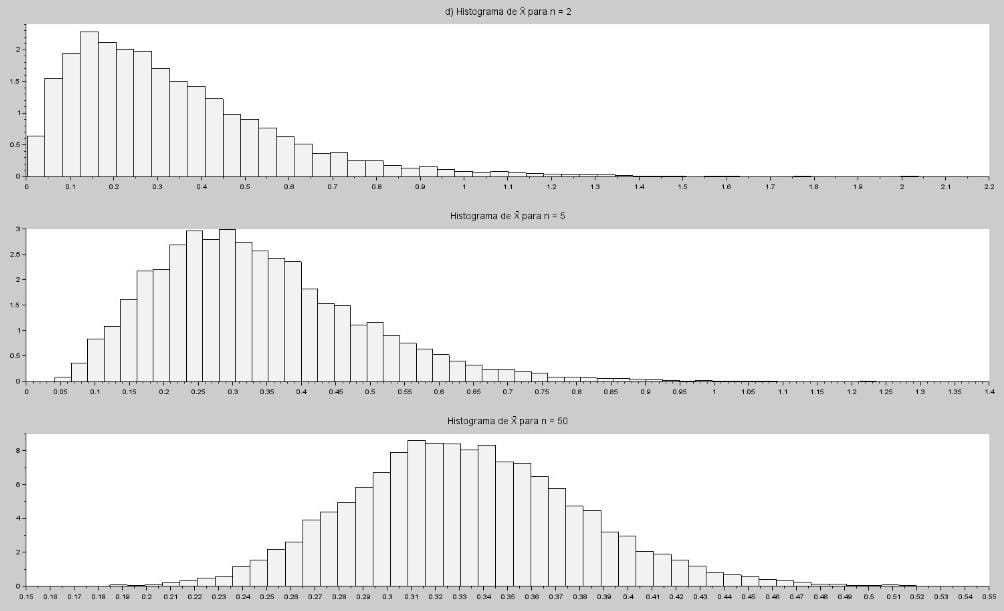
\includegraphics[width=0.80\linewidth]{figures/grafico2_hist_medias.jpg}
        \caption*{Conforme $n$ aumenta, a distribuição de $\bar{X}$ se aproxima da Normal e sua variância diminui.}
    \end{figure}
\end{frame}

% Slide 6: Código e Resultados da alternativa 'e'
\begin{frame}[fragile]{e) Estatísticas das Médias Amostrais}
    \textbf{e) Calcule a média e o desvio padrão das 10.000 médias amostrais ($\bar{X}$) para cada $n$.}

\begin{lstlisting}
// Média das médias amostrais
media_Xbar2 = mean(Xbar2)   // Resultado esperado: ~0.333
media_Xbar5 = mean(Xbar5)   // Resultado esperado: ~0.333
media_Xbar50 = mean(Xbar50) // Resultado esperado: ~0.333

// Desvio padrão das médias amostrais
dp_Xbar2 = stdev(Xbar2)     // Esperado: (1/3)/sqrt(2) ~ 0.2357
dp_Xbar5 = stdev(Xbar5)     // Esperado: (1/3)/sqrt(5) ~ 0.1490
dp_Xbar50 = stdev(Xbar50)   // Esperado: (1/3)/sqrt(50) ~ 0.0471
\end{lstlisting}
\end{frame}

% Slide 7: Enunciado da alternativa 'f'
\begin{frame}{f) O Teorema do Limite Central (TLC)}
    \textbf{f) Com base nos resultados, enuncie o Teorema do Limite Central e explique como ele se aplica a este experimento.}
    
    \textbf{Enunciado do TLC:}
    \begin{quote}
        Dada uma população com média $\mu$ e desvio padrão $\sigma$ finitos, a distribuição das médias amostrais ($\bar{X}$) de amostras de tamanho $n$ retiradas desta população aproxima-se de uma distribuição Normal com média $\mu$ e desvio padrão $\sigma/\sqrt{n}$, à medida que $n$ se torna suficientemente grande.
    \end{quote}
    
    \textbf{Aplicação ao experimento:}
    \begin{itemize}
        \item A distribuição original é fortemente assimétrica (Gráfico 1).
        \item No entanto, os histogramas das médias amostrais mostram que, à medida que $n$ aumenta de 2 para 50, a distribuição de $\bar{X}$ torna-se cada vez mais simétrica e com formato de sino, ou seja, Normal.
        \item As médias das $\bar{X}$ mantiveram-se em torno de $\mu = 1/3$, e os desvios padrão diminuíram visivelmente, aproximando-se de $\sigma/\sqrt{n}$, confirmando as previsões do teorema.
    \end{itemize}
\end{frame}
